%----------------------------------------------------------------------------------------
%	SLIDE 4.
%----------------------------------------------------------------------------------------
\begin{frame}
\frametitle{Szálak futása}

\begin{columns}
	\column{0.55\linewidth}
	\begin{block}{Szálak kezelése}
		{\small
		\begin{enumerate}
			\item Programnyelv szintjén
			\begin{itemize}
				\item A felhasználó dönti el, hogy a program melyik részét és hogyan bontja szálakra.
			\end{itemize}
			\item Operációs rendszer szintjén
			\begin{itemize}
				\item Az OS szálkezelője dönti el a szálak futtatásának ütemét
			\end{itemize}
		\end{enumerate}
		}
	\end{block}

	\begin{block}{Párhuzamos futás}
		{\small
		\begin{itemize}
			\item Több mag, mint szál esetén ténylegesen párhuzamosan futnak
			\item Több szál, mint mag esetén a CPU periodikusan váltogat közöttük
		\end{itemize}
		}
	\end{block}
	
	\column{0.4\linewidth}
	\begin{figure}
		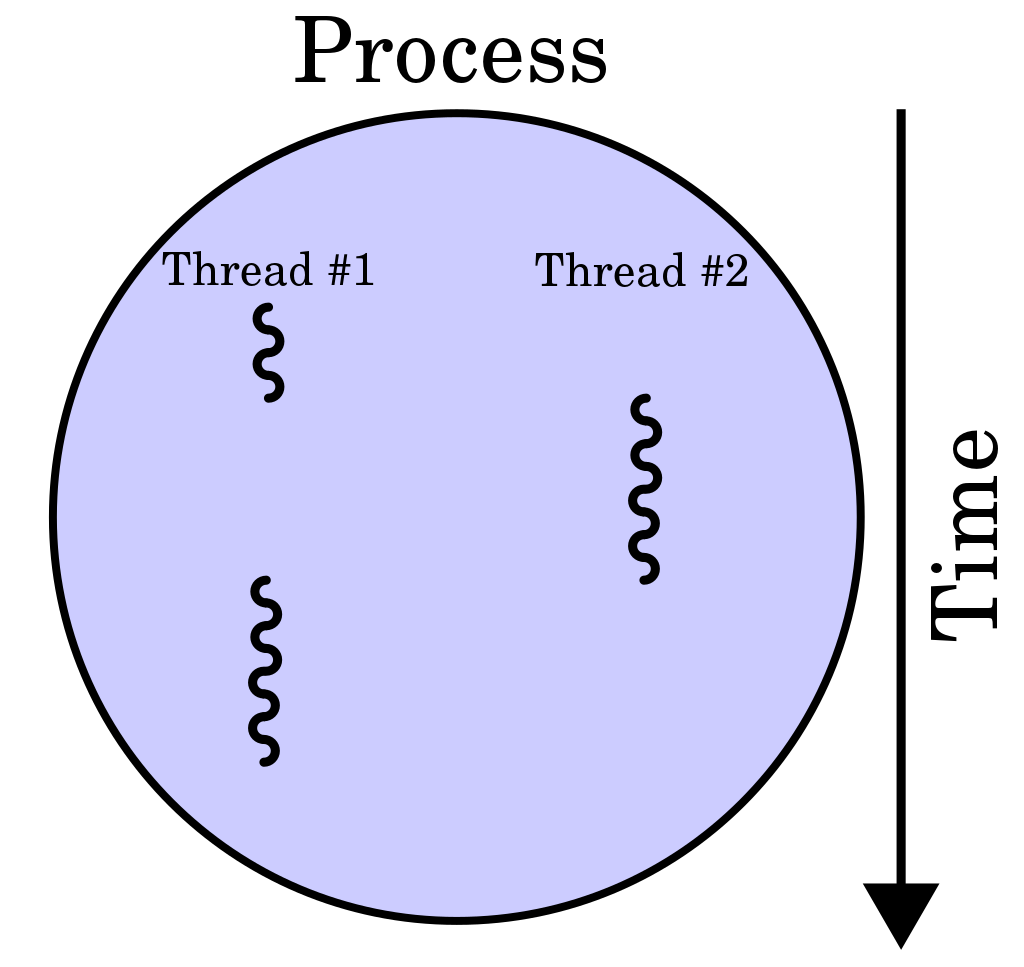
\includegraphics[width=\textwidth]{img/thread-serial.png}
		{\hspace*{\fill}\tiny\textit{Forrás: Cburnett, Wikipedia}}
	\end{figure}
	
\end{columns}

\end{frame}